% !TeX spellcheck = de_CH
%%%%%%%%%%%%%%%%%%%%%%%%%%%%%%%%%%%%%%%%%%%%%%%%%%%%%%%%%%%%%%%%%
%  _____   ____  _____                                          %
% |_   _| /  __||  __ \    Institute of Computitional Physics   %
%   | |  |  /   | |__) |   Zuercher Hochschule Winterthur       %
%   | |  | (    |  ___/    (University of Applied Sciences)     %
%  _| |_ |  \__ | |        8401 Winterthur, Switzerland         %
% |_____| \____||_|                                             %
%%%%%%%%%%%%%%%%%%%%%%%%%%%%%%%%%%%%%%%%%%%%%%%%%%%%%%%%%%%%%%%%%
%
% Project     : BA Welti Keller
% Title       : 
% File        : software.tex Rev. 00
% Date        : 15.09.2014
% Author      : Tobias Welti
%
%%%%%%%%%%%%%%%%%%%%%%%%%%%%%%%%%%%%%%%%%%%%%%%%%%%%%%%%%%%%%%%%%

\chapter{Software-Konzept}\label{chap.software}


\section{Software-Stack}\label{sec.sw_stack}
\todo{Glossar: Bus, Mikroprozessor, A/D-Wandler, Pin, }

\subsection{Überblick}\label{subsec.sw_ueberblick}

\begin{figure}[H]
	\centering
		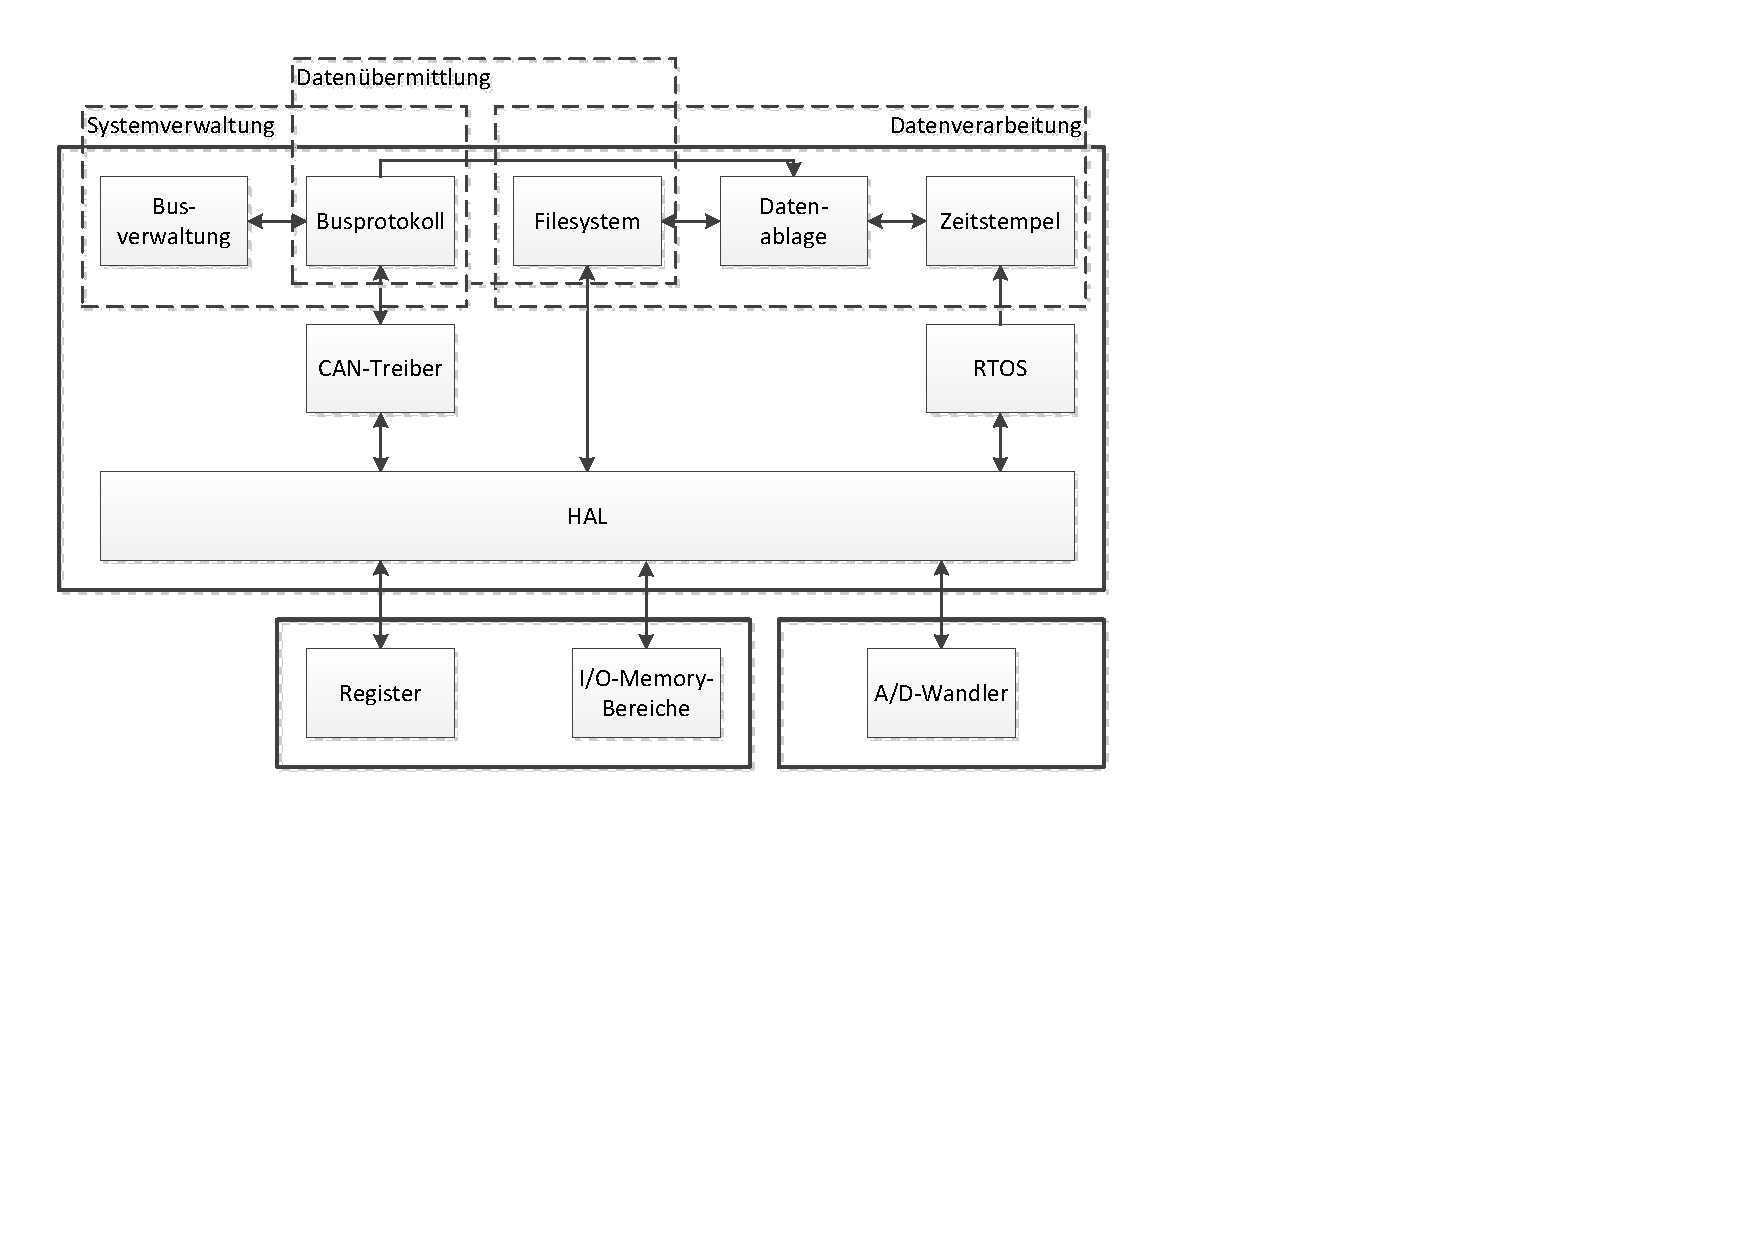
\includegraphics[width=0.8\textwidth]{images/visio/Softwarestack_Logger.pdf}
	\caption{Softwarestack des \gls{logger}s.}
	\label{fig.sw_logger}
\end{figure}

\begin{figure}[H]
	\centering
		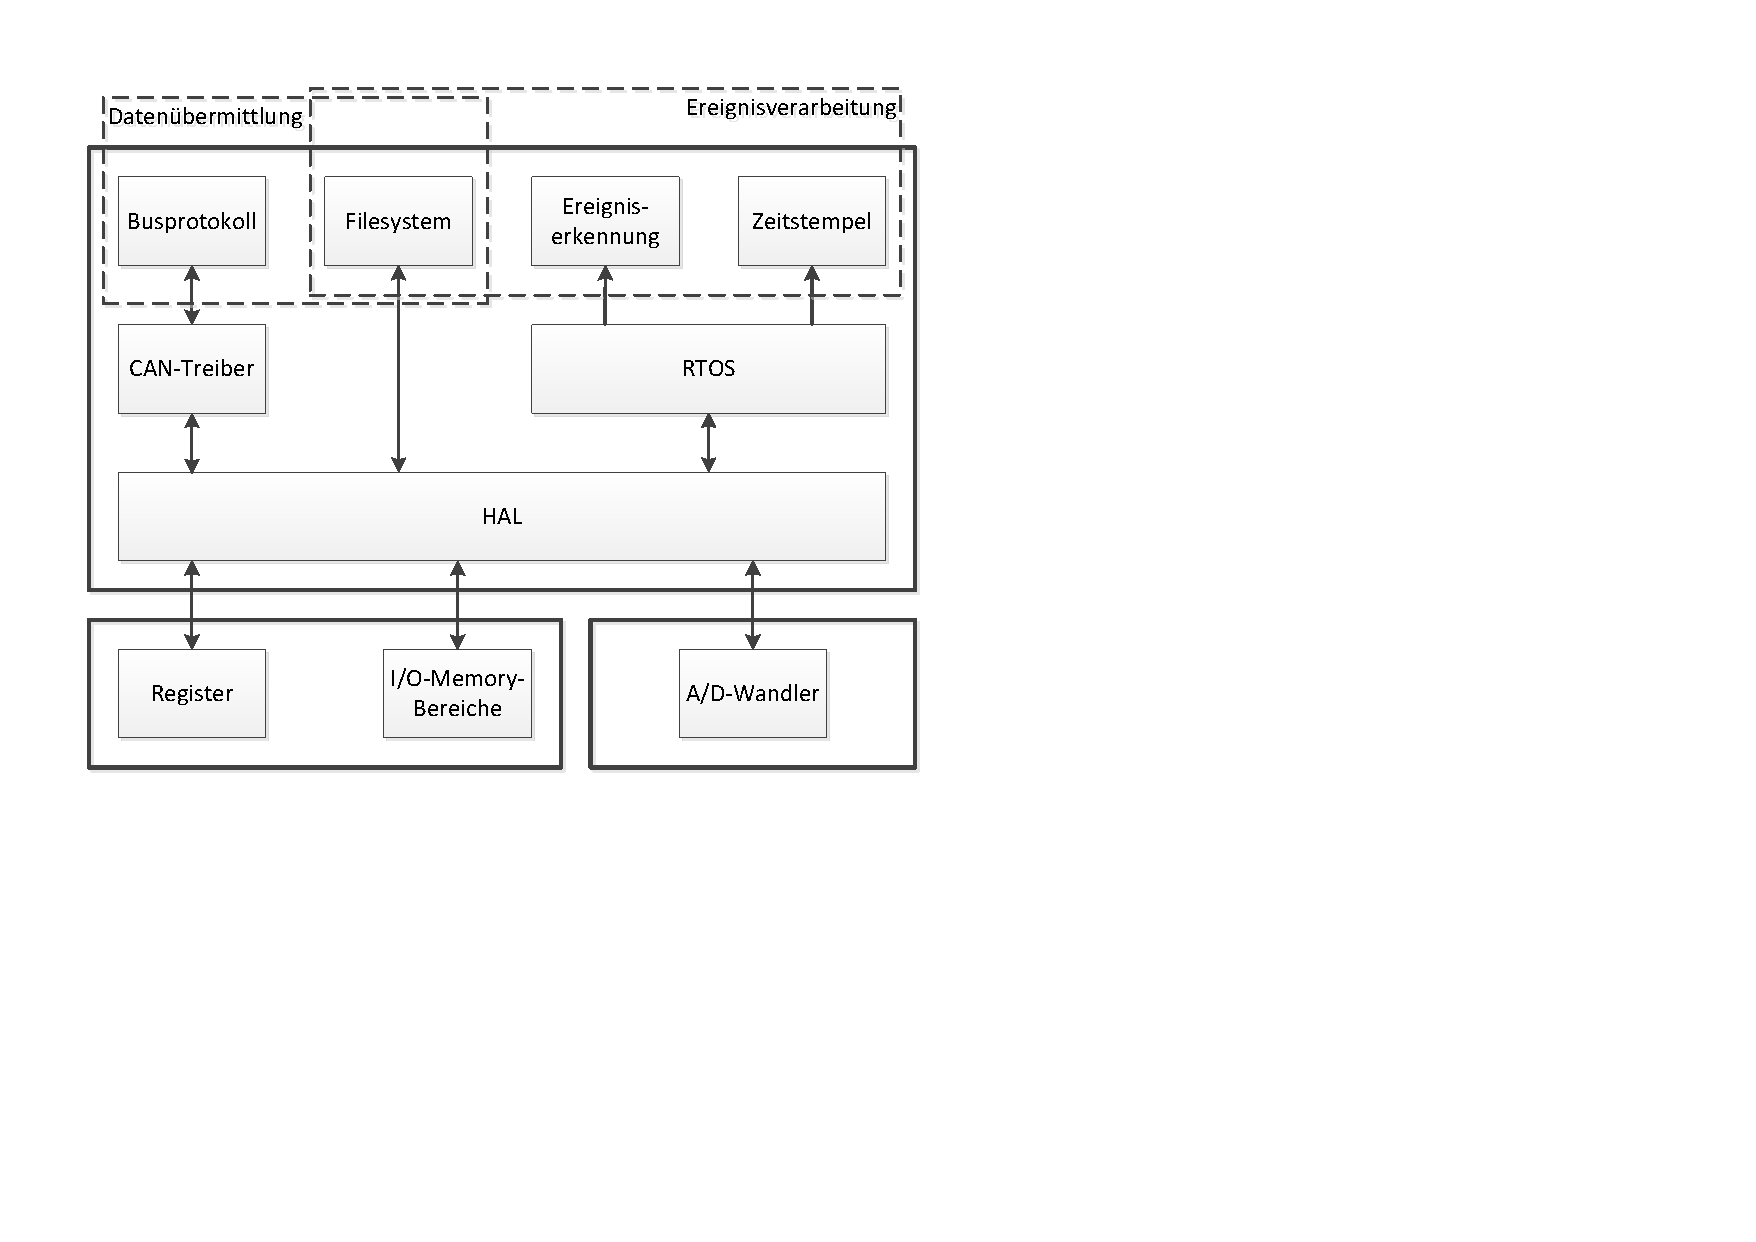
\includegraphics[width=0.8\textwidth]{images/visio/Softwarestack_Sensor.pdf}
	\caption{Softwarestack der \gls{sensoreinh}.}
	\label{fig.sw_sensor}
\end{figure}



\subsection{Messdatenerfassung}\label{subsec.sw_messen}
Der NXP LPC4088 Mikroprozessor verfügt über einen 12-bit A/D-Wandler, der über einen Multiplexer auf acht Pins messen kann. Auf dem verwendeten Quickstart-Board stehen 6 Pins für A/D-Wandlung zur Verfügung. Für die geplante Anwendung reicht ein A/D-Eingang, da der Beschleunigungs-\gls{sensor} die Beschleunigung nur auf einer Achse misst. Der A/D-Wandler des NXP LPC4088 wird mit einer Abtastrate von 10~kHz betrieben. Falls höhere Abtastraten nötig sind, kann der A/D-Wandler mit bis zu 400~kHz betrieben werden.



\subsection{Ereigniserkennung}\label{subsec.sw_ereignis}
Vom WSL wurde die Ereigniserkennung bisher mittels Hilbert-Transformation gelöst. Die Hilbert-Transformation liefert die umhüllende Kurve des gemessenen Signals. Überschreitet die Umhüllende den \gls{threshold}, markiert dies den Start eines neuen \gls{ereignis}ses. Fällt die Umhüllende unter den \gls{threshold}, ist das \gls{ereignis} beendet. Um den Rechenaufwand der Hilbert-Transformation zu umgehen, lösen wir die Ereigniserkennung einfacher.
\todo{FSM-figur anpassen auf neue Stati}
\begin{figure}[H]
	\centering
		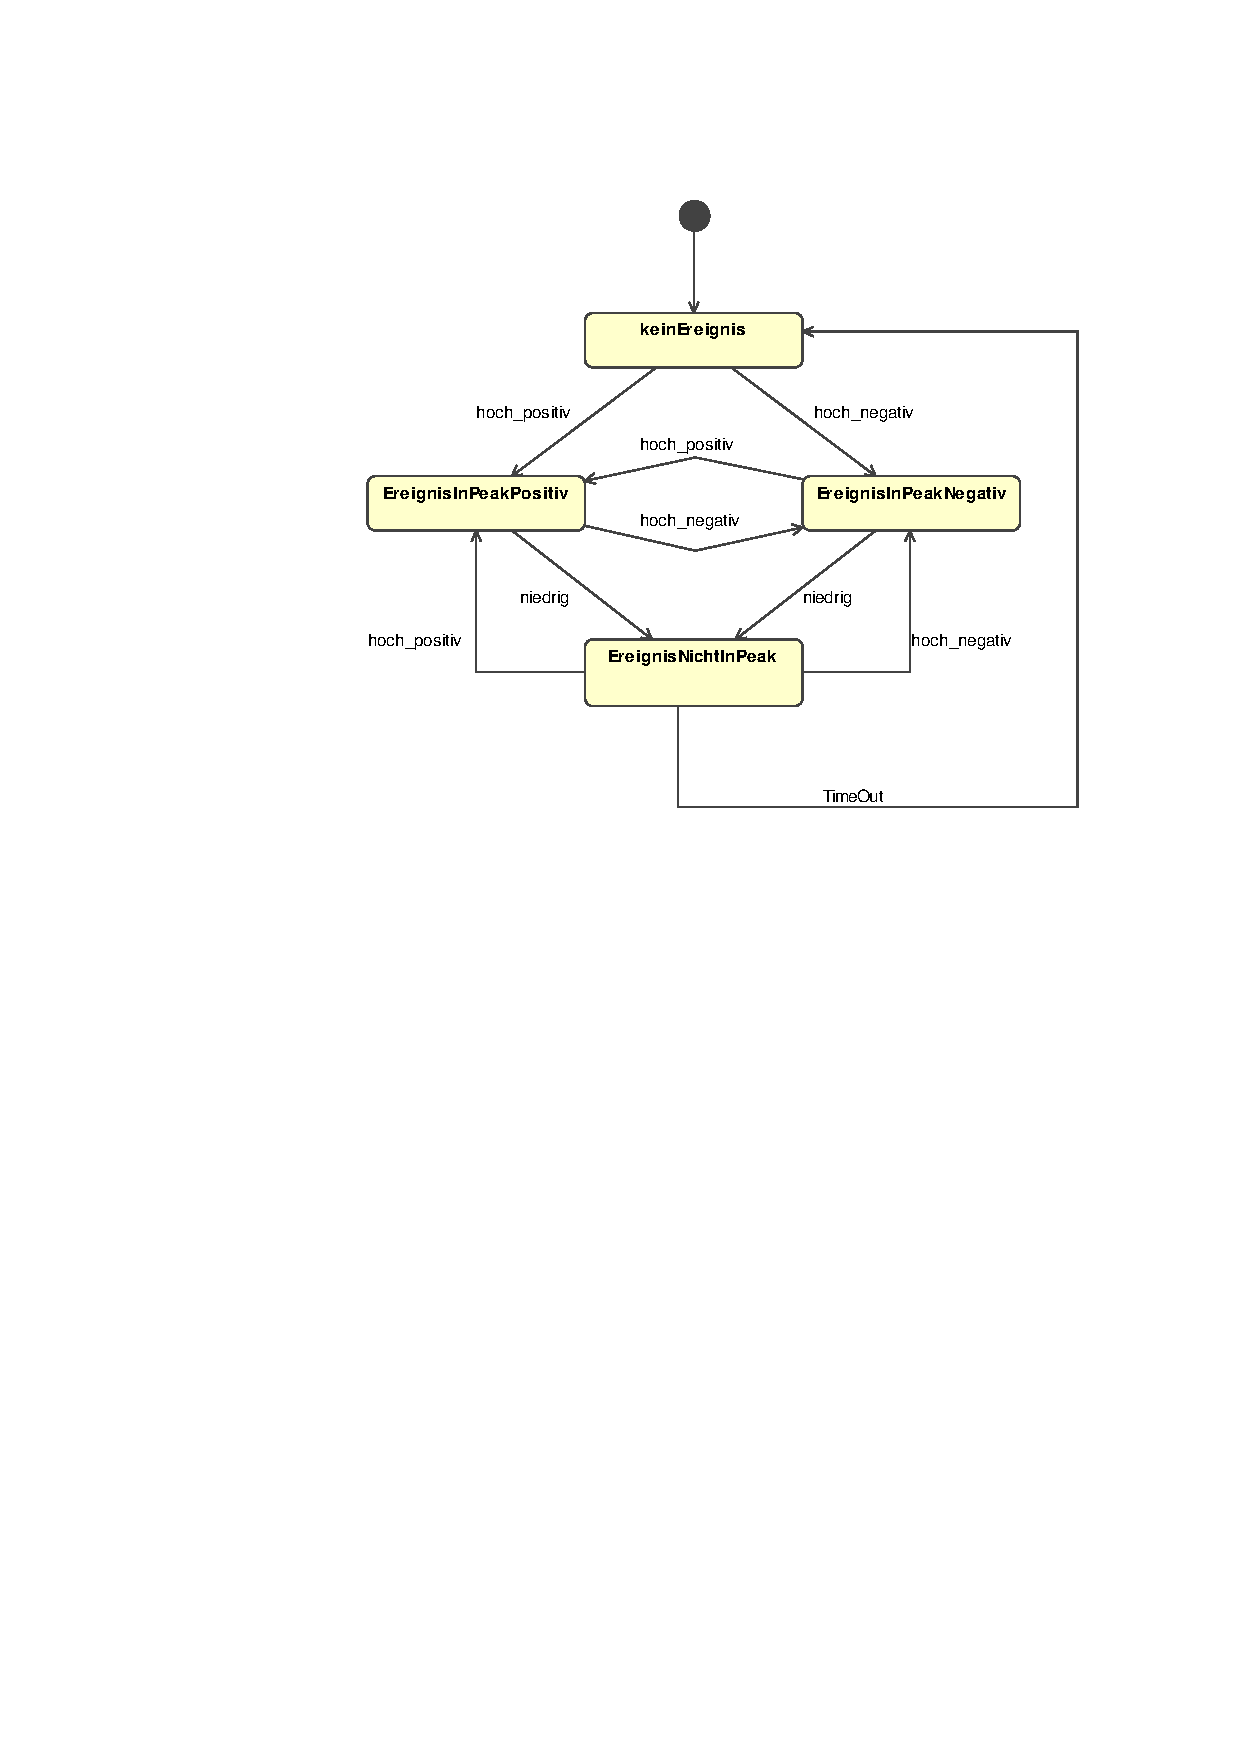
\includegraphics[width=0.6\textwidth]{images/magicdraw/Ereigniserkennung.pdf}
	\caption{Zustandsmaschine der Ereigniserkennung.}
	\label{fig.fsm_impact_detection}
\end{figure}

\todo{Ereigniserkennung beschreiben, welche Parameter können konfiguriert werden}
\todo{Zusammenhänge A/D-Wandlung und Ereigniserkennung und Übertragung beschreiben}
\todo{Verschiedene Betriebsmodi mit Grafiken beschreiben}
\todo{Berechnungen, in welchem Modus wie lange gemessen werden kann, und wie lange ein \gls{sensor} mit dem vorhandenen Speicher die Resultate zwischenspeichern kann. Allenfalls ein System erwähnen, das automatisch zwischen verschiedenen Modi hin- und herschalten kann. (Ist allerdings heikel). Wie viele \glspl{sensor} können in welchem Modus gleichzeitig am System betrieben werden, bei welcher Ereignisrate ist Schluss mit Busbandbreite.}

\subsection{\gls{timestamp}}\label{subsec.sw_timestamp}
\todo{Timestamp beschreiben, Rechnung über die Dauer der eindeutigen Zuweisung.}

\subsection{Verwaltung der Messstation}\label{subsec.sw_busverwaltung}
\todo{Busverwaltung beschreiben}

\begin{figure}[H]
	\centering
		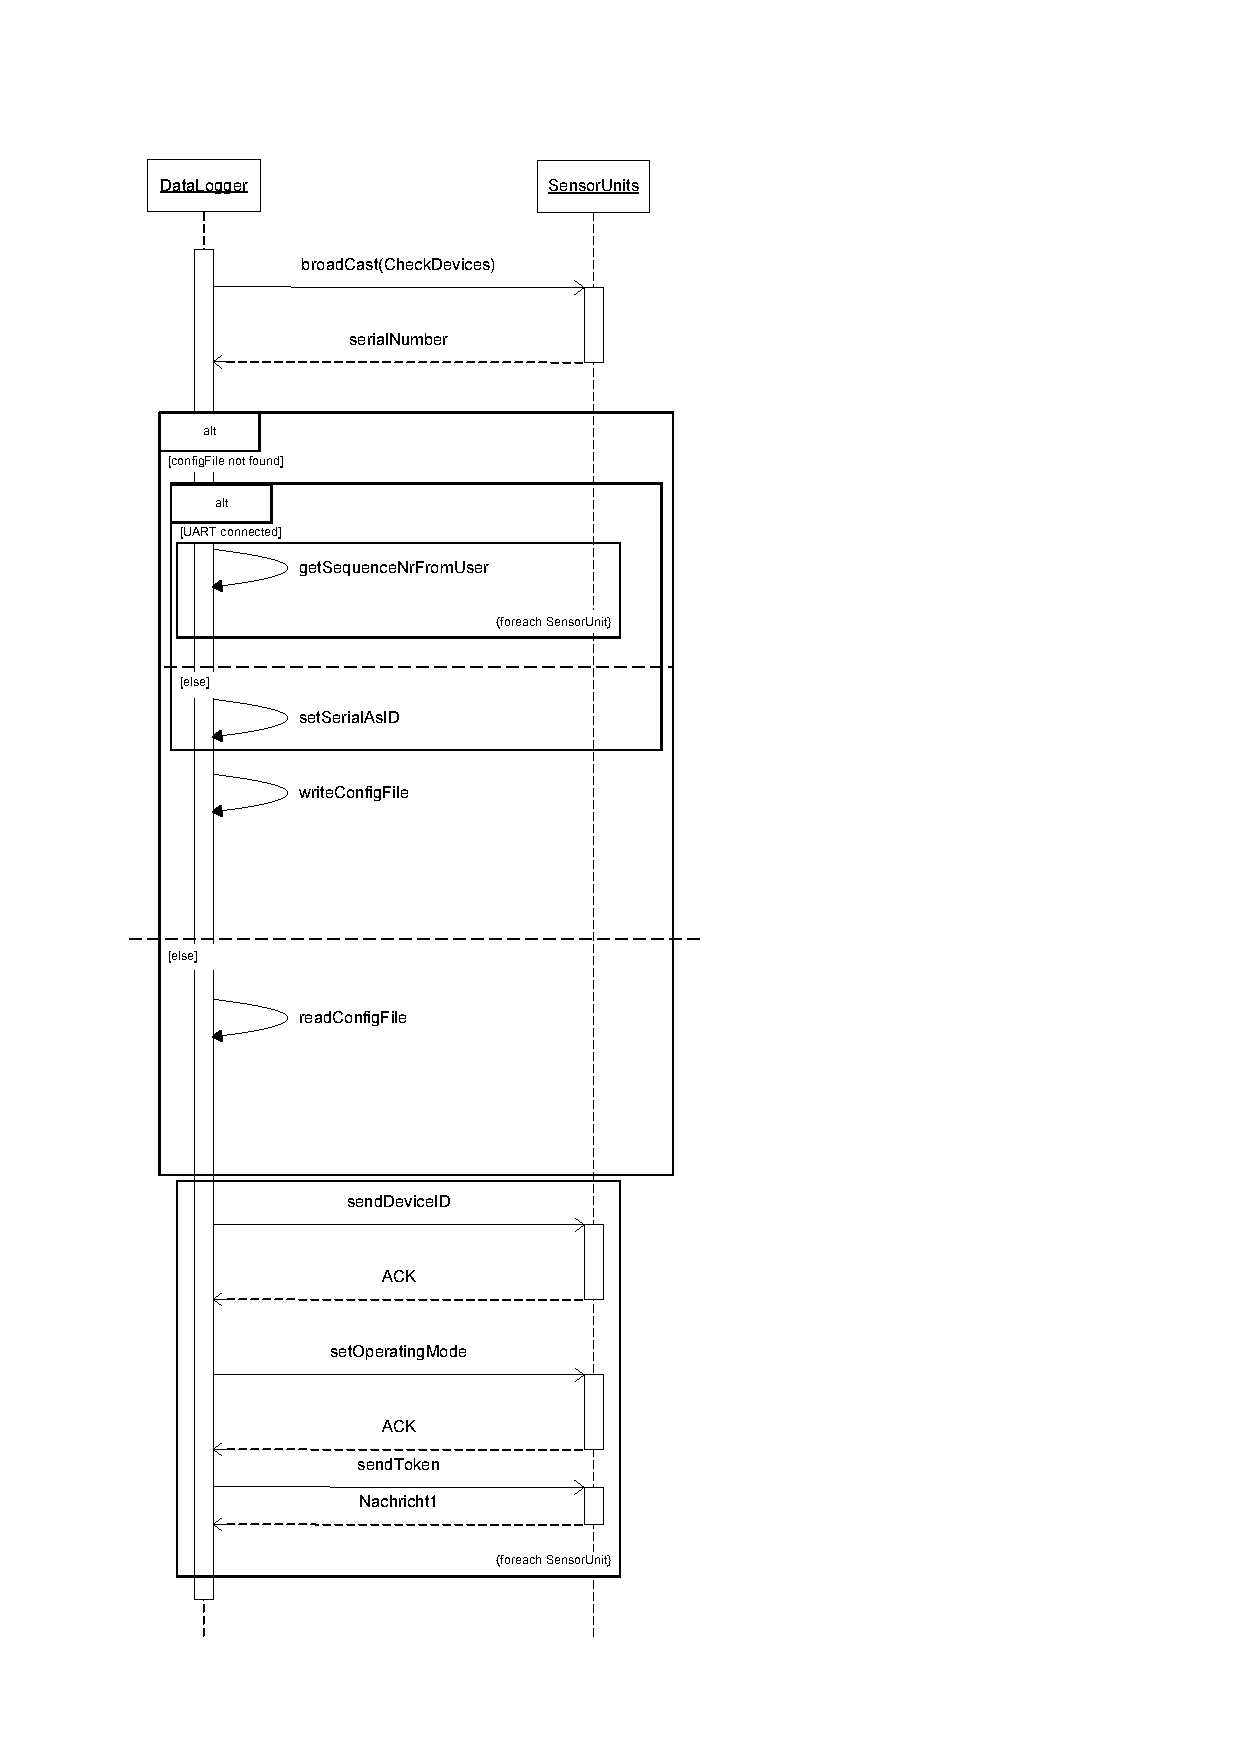
\includegraphics[height=0.9\textheight]{images/magicdraw/StartUpSequenz.pdf}
	\caption{Sequenzdiagramm des Startupvorgangs der Messstation.}
	\label{fig.seq_startup}
\end{figure}

\todo{Figur \ref{fig.seq_startup} aufteilen auf zwei Seiten. (PDF-crop)}

\subsection{Busprotokoll}\label{subsec.sw_busprotokoll}
\todo{Busprotokoll austüfteln. Darstellung siehe HW-Konzept Rioxo, genaue Beschreibung der Nachrichtentypen. Timestamp der einzelnen Peaks bezieht sich auf Offset vom Beginn des Impacts.}
\todo{Kommunikationsdiagramm Bushandler}
\todo{Interrupt-System des Bushandlers aufführen}

\subsection{Filesystem}\label{subsec.sw_filesystem}
\todo{Texten}
\todo{Frage: wird für jeden \gls{sensor} ein eigenes File geführt? Kann man alle Files offen lassen oder ist das keine gute Idee? Was ist besser, jedes mal das File-Ende zu suchen um neues anzuhängen?}

\subsection{UART-Kommandozeile}\label{subsec.sw_uart}
\todo{Dokumentation über die Kommandos, wird später für die Bedienungsanleitung gebraucht}

\section{Funktionalität}\label{sec.sw_funktionalitaet}
\todo{Texten}

\section{Konfiguration}\label{sec.sw_konfiguration}
\todo{Hier eine Art Bedienungsanleitung zur Konfiguration geben. Welches Kommando hat was 
zur Folge? (Wird Datenerfassung neu gestartet, werden allenfalls andere \glspl{sensor} deaktiviert 
etc.}